\documentclass{article}
\usepackage{amsmath}
\usepackage{hyperref}
\usepackage{tikz}
\usepackage{graphicx} 
\usepackage{siunitx}  
\usepackage{circuitikz}

\begin{document}

\title{UHF PA Design Exercise}
\maketitle

This document is a record of some experiments with a two stage PA board using a generic gain block as a driver, and RDMUS01 mosfet final stage, conducted in July 2026 by Tibor, with David taking notes.  Some details of the module including a complete schematic are presented on the \href{https://ka7oei.blogspot.com/2023/04/exploring-1-930mhz-2w-rf-broadband.html}{KA7OEI blog}. The aim was to develop a stable, 1W PA for 400-450 MHz (including the Ham 70 \si{cm} band). The general approach was:
\begin{itemize}
\item Start with the generic unmatched, broadband module (untuned 50 \si{\ohm} matches throughout).
\item Add a $R_{deg}=20$ \si{\ohm} degeneration resistor across the mosfet gate to ensure stability (and the cost of some gain). Reducing this to 10 ohms resulted in insufficient drive to the final stage.
\item Build an interstage match to transform the 50 ohm driver output impedance to 20 \si{\ohm} mosfet gate impedance.
\item We chose $V_{dd}=7.6$ \si{V} such that a 2x swing on the mosfet output will be well less than $V_{vddmax}=25$ \si{V}.
\item We chose an output impedance for the mosfet of 20 \si{\ohm} to obtain 1W.
\item We designed an output match for 20 to 50 \si{\ohm}. This was initially a L network, we later experimented with a $\pi$ network, which had better harmonic suppression.
\end{itemize}

General Tips:
\begin{itemize}
\item Use vaseline as a non-toxic thermal grease between mosfet and heatsink.
\item Use physically large, high $Q\approx100$ commercial inductors for matching. Not hand wound air core or wire loops, as they are excellent antennas.
\item Use 100 \si{pF} bypass capacitors rather than 1 \si{nF}, as lower impedance. 
\item Matching C in output stage was adjusted to achieve flat gain between $400-450$ \si{MHz}.
\end{itemize}

\begin{figure}[h]
    \centering
\begin{circuitikz}[american, scale=1.1, transform shape]

    % ==========================================
    % 1. DRIVER STAGE (Generic Gain Block)
    % ==========================================
    % Place the amplifier block at the start
    \draw (-4.5, 0) node[buffer] (Driver) {};
    \draw (-5.5, 0) node[left] {RF IN} -- (Driver.west);
    
    % Transistor Node
    \draw (0,0) node[nmosd] (Q) {};

    % ==========================================
    % 2. INTER-STAGE MATCHING
    % ==========================================
    % Output of Driver connects to an interstage matching C
    \draw (Driver.out) -- (-3.5,0) node[circle, fill, inner sep=1pt] (driver_out) {}
                       to[C, l=$C_{\text{1}}$] (-1.5, 0) -- (Q.gate);
                      
    % Shunt L to ground for impedance tuning, DC block to AC ground
    \draw (driver_out) to[L, l_=$L_{\text{1}}$] (-3.5, -2) node[circle, fill, inner sep=1pt] (driver_vdd) {}
                    to[C, l_=$C_{\text{b1}}$] (-2.5, -2) node[circle, fill, inner sep=1pt] (gnd1) {};
    \draw (gnd1) to (-2.5, -3) node[ground] {};

	\draw (driver_vdd) to[L, mirror, l_=$RFC$] (-5.5, -2) to[short] (-6, -2) node[left] {$V_{\text{dd}}$};

	% Add the blue current arrow
    \draw[->, blue, thick] (-2.35, -0.5) arc (90:-180:0.5);
    \node[blue] at (-2.35, -1) {$i_{in}$};

    % ==========================================
    % 3. FINAL OUTPUT STAGE (RD01MUS2)
    % ==========================================
    \node[right=0.2cm, font=\bfseries] at (Q.text) {Q1};
    \node[right=0.2cm, yshift=-0.4cm, font=\small] at (Q.text) {RD01MUS2};

    % Ground the Source
    \draw (Q.source) -- (0,-1) node[ground] {};

    % Connect Inter-stage to Gate via Bias Node
    %\draw (In_node) -- (Q.gate);
    \draw (-1.5, 0) node[circle, fill, inner sep=1pt] (G_bias) {};
    
    % Gate Bias Feed
    \draw (G_bias) -- (-1.5, 0) to[R, l=$R_{\text{deg}}$] (-1.5, -2.0) 
          node[circle, fill, inner sep=1pt] (Vgg_node) {}
          to[short] (-1.0, -2.0) node[right] {$V_{\text{gg}}$};
	\draw (Vgg_node) to [C, l=$C_{\text{b2}}$] (-2.5,-2);
	 
    % Drain Output Side (DC Feed & Output Matching)
    \draw (Q.drain) -- (0,1) node[circle, fill, inner sep=1pt] (D_node) {};
    
    % DC Supply Feed via RF Choke
    \draw (D_node) to[L, mirror, l=$RFC$] (0, 2.5) to[short] (0, 3) node[above] {$V_{\text{dd}}$};

    % Output Matching Network
    \draw (D_node) to[C, l=$C_{\text{2}}$] (2.5,1) node[circle, fill, inner sep=1pt] (Out_node) {};
    \draw (Out_node) to[L, l=$L_{\text{2}}$] (2.5,-0.5) node[ground] {};
    \draw (Out_node) to[short] (3,1) node[right] {RF OUT};

\end{circuitikz}

\caption{Two stage prototype PA. An input match is formed from $C_1$ and $L_1$, and an output match by $C_2$ and $L_2$, both with high pass topologies. $R_{deg}$ is the degeneration resistance that ensures stability. $V_{gg}$ is the DC gate bias. $C_{b1}$ and $C_{b2}$ are DC blocks. The layout should make the current loop $i_{in}$ as small as possible.}
    \label{fig:my_image_label}
\end{figure}

\begin{figure}[h]
    \centering              
    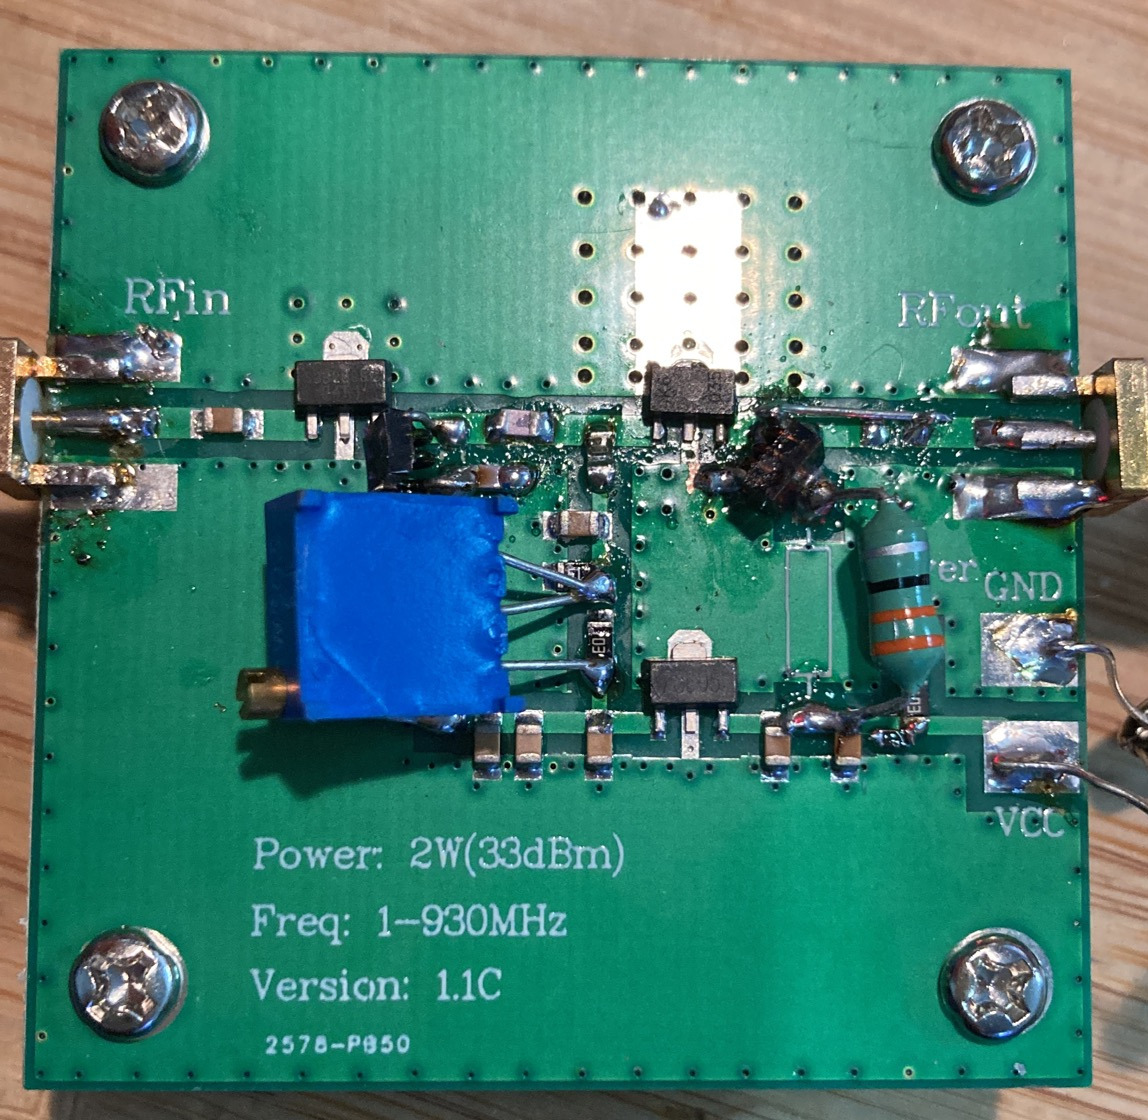
\includegraphics[width=0.6\textwidth]{board1}
    \caption{Two stage PA PCB used for prototyping, modified to have an interstage and final stage high pass matches. Trimmer provides $V_{gg}$ gate bias adjustment.}
    \label{fig:my_image_label}
\end{figure}

\begin{figure}[h]
    \centering              
    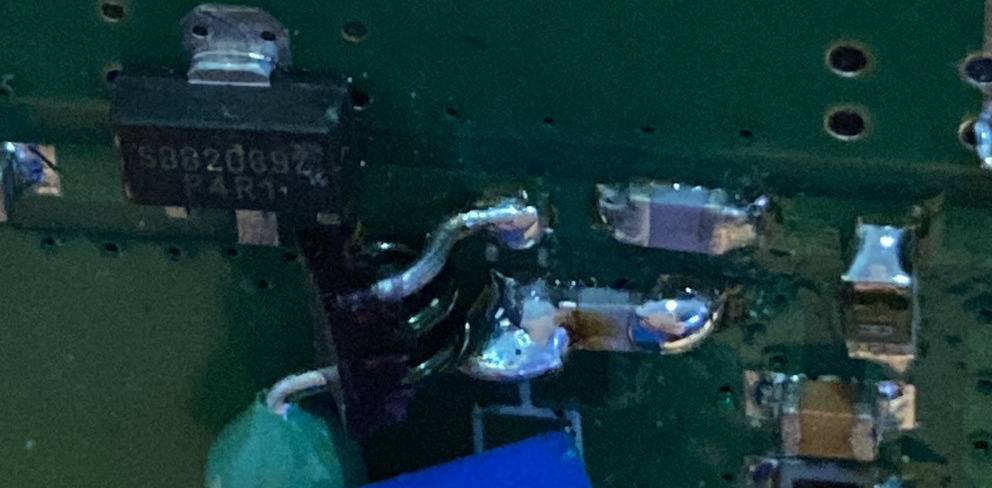
\includegraphics[width=0.6\textwidth]{board2}
    \caption{Interstage match layout: $C_{b1}$ (lower middle) and $C_{b2}$ (lower right) ground nodes connected close together to minimise current loop $i_{in}$. $R_{deg}$ is on RHS, $C_1$ in middle.}
    \label{fig:my_image_label}
\end{figure}

\begin{figure}[h]
    \centering              
    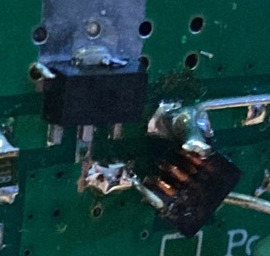
\includegraphics[width=0.6\textwidth]{board3}
    \caption{Output shunt matching component (in this iteration an inductor) is connected directly to the mosfet source pin to minimise the current loop. A better ground connection was later found to be the plane area (top), which is connected to the pad on the bottom of the mosfet.}
    \label{fig:my_image_label}
\end{figure}

\begin{figure}[h]
    \centering              
    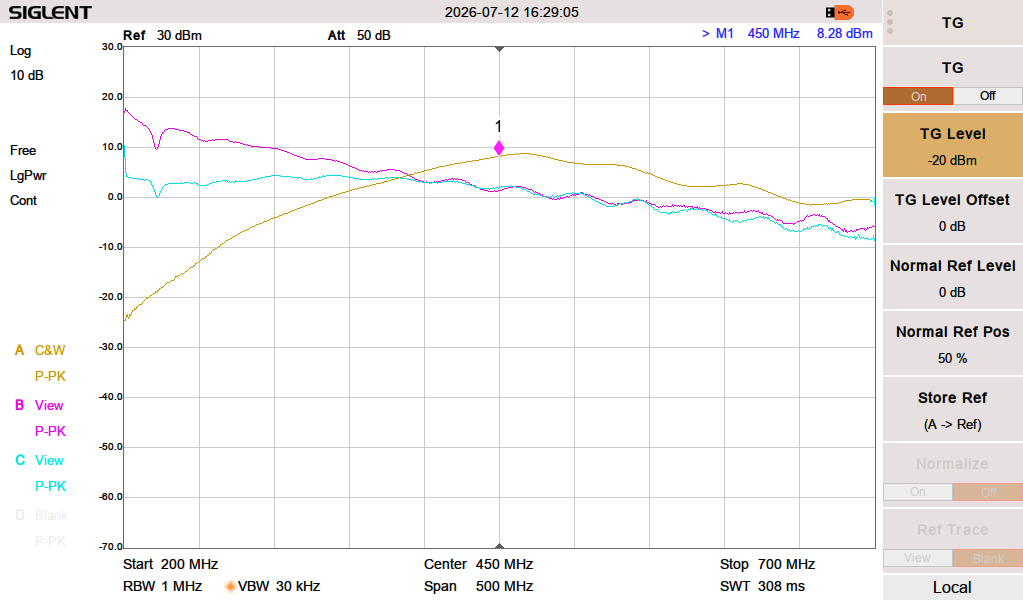
\includegraphics[width=1.2\textwidth]{tracking1}
    \caption{Purple unmodified original, no matches, straight through 50 ohm design. Blue is with gate degeneration 10 ohm resistor, but no matching. Yellow is the completed first prototype with high pass interstage match and high pass output match.}
    \label{fig:my_image_label}
\end{figure}

\begin{figure}[h]
    \centering              
    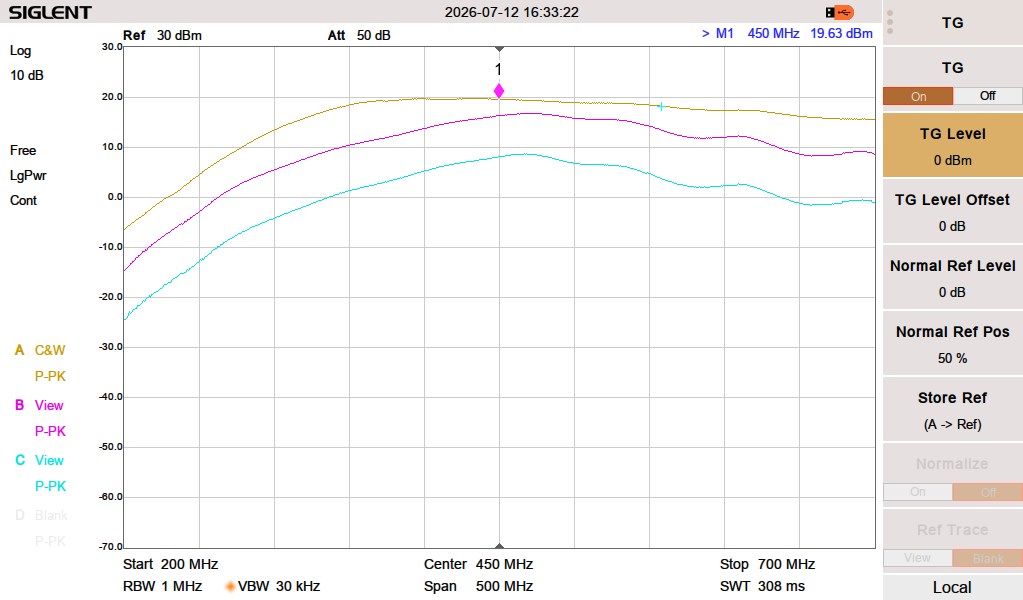
\includegraphics[width=1.2\textwidth]{tracking2}
    \caption{Performance across drive levels. Blue -20 \si{dBm}, pink -10 \si{dBm}, yellow 0 \si{dBm} drive (compressed). When compressed, power gain is 30 \si{dB}, when uncompressed 36 \si{dB}.}
    \label{fig:my_image_label}
\end{figure}

\end{document}
